\begin{figure}[H]
    \centering
    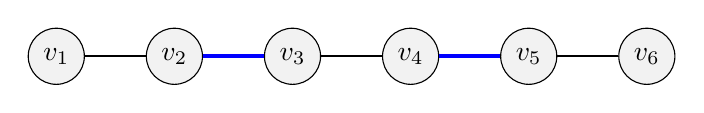
\begin{tikzpicture}[node distance=1.5cm, every node/.style={circle, draw, fill=gray!10, minimum size=0.7cm}]
        % Wierzchołki
        \node (v1) {$v_1$};
        \node (v2) [right of=v1] {$v_2$};
        \node (v3) [right of=v2] {$v_3$};
        \node (v4) [right of=v3] {$v_4$};
        \node (v5) [right of=v4] {$v_5$};
        \node (v6) [right of=v5] {$v_6$};

        % Krawędzie nienależące do skojarzenia (zwykłe)
        \draw[thick] (v1) -- (v2);
        \draw[thick] (v3) -- (v4);
        \draw[thick] (v5) -- (v6);

        % Krawędzie należące do skojarzenia (pogrubione, niebieskie - spójne z Rys 4.)
        \draw[line width=1.5pt, blue] (v2) -- (v3);
        \draw[line width=1.5pt, blue] (v4) -- (v5);
    \end{tikzpicture}
    \caption{Przykład ścieżki powiększającej. Pogrubione (niebieskie) linie to krawędzie należące do aktualnego skojarzenia $M$, natomiast cieńsze (czarne) do niego nie należą. Skrajne wierzchołki $v_1$ i $v_6$ są wolne (nieskojarzone). Zamiana ról krawędzi na ścieżce zwiększy rozmiar skojarzenia o jeden.}
    \label{rys:sciezka_powiekszajaca}
\end{figure}